\todo{per ogni sezione chiedere a Vittoria e Ginevra come li userebbero in clinica}
\section{Implemented Tool} \label{sec:implemented-tool}
\subsection{Overview}
The system often referenced and shown in some detail in Sec. \ref{sec:novel-contributions} is a proof-of-concept terminal-based tool that was developed in order to test the hypotheses laid out in Chap. \ref{chap:introduction} and in Sec. \ref{sec:methodology-introduction}.
The defining motivation was to have a working software that could be given to a number of clinicians at the ICP (see Subsec. \ref{subsec:istituto-cantonale}) in order to have them test the theoretical questions, defined in \ref{sec:response}, that are at the core of this thesis.
Being this only a prototype, the implementation was carried out using Python 3.6, as this was the language that let me best focus on rapid development, due to my familiarity with it and to its vast array of available libraries.

Despite never meaning to be a production software, particular care was taken in the design of the interface, as described in Subsec. \ref{subsec:algorithms-novel}, in line with the spirit of this work that is to study human-machine interaction.

In the following, the various interaction modalities with the tool are presented using screenshots.
The basic methods underlying the tool have already been discussed at length in Sec. \ref{sec:novel-contributions} so the current examination will focus on the interface, as perceived by the user, and how these methods have been incorporated into the system.
Where relevant, the information and descriptions given in Sec. \ref{sec:novel-contributions} will be integrated.

Fig. \ref{fig:sw_0} shows the first screen presented during use.
The user has the possibility of inputting the path to the dataset to use, or to accept the hardcoded one, that in this case is the one described in Sec. \ref{sec:data-set}.
Next, the number of entries before and after preprocessing are shown; the data set in question see its number of valid records go from 3217 to 2873, after the rules of Tab. \ref{tab:datasetpreprocess} have been applied.
The \enquote{Inspect data set} and \enquote{ML} options are only for testing and validation purposes; the former surfaces a pair of options to visualise the distribution of the data set's variables' values and the normalised entropies, the latter runs the Machine Learning tests that will be discussed in Sec. \ref{sec:prediction-evaluation}.
The main focus will be the \enquote{Build Bayesian Network} section as this is where all the methods discussed in Chap. \ref{chap:methodology} are to be found.
Selecting this option automatically uses pomegranate to construct a Bayesian Network model of the selected data set.
The user is then shown what is the main menu of the application, as can be seen in Fig. \ref{fig:sw_1}.

\begin{figure}[htbp]
\centerline{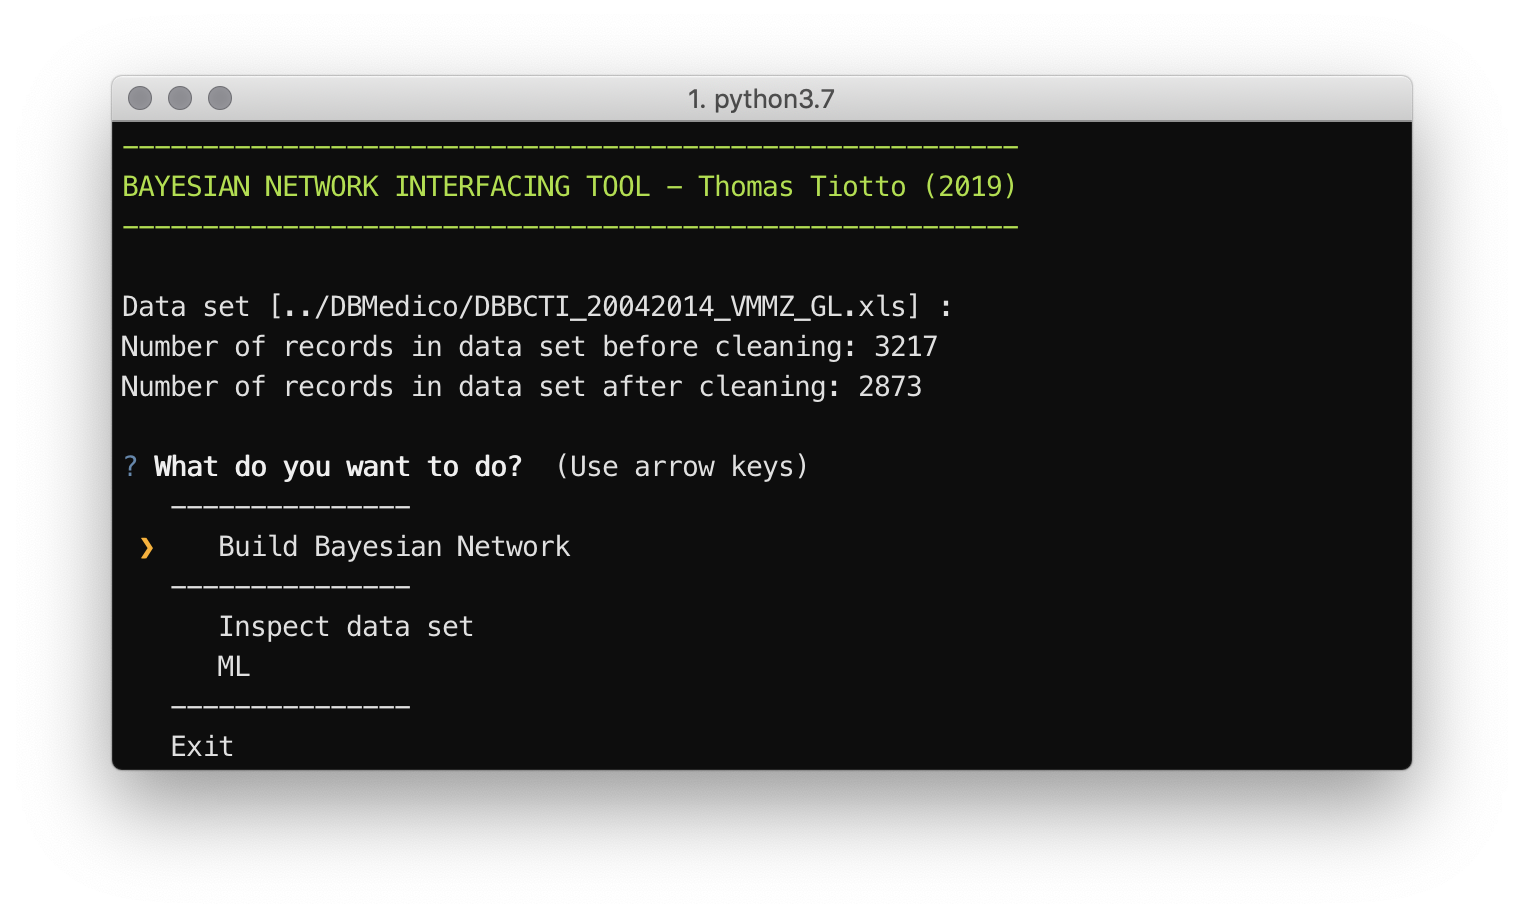
\includegraphics[width=\columnwidth]{results/images/sw_0}}
\caption{Initial screen in the developed tool.}
\label{fig:sw_0}
\end{figure}

\begin{figure}[htbp]
\centerline{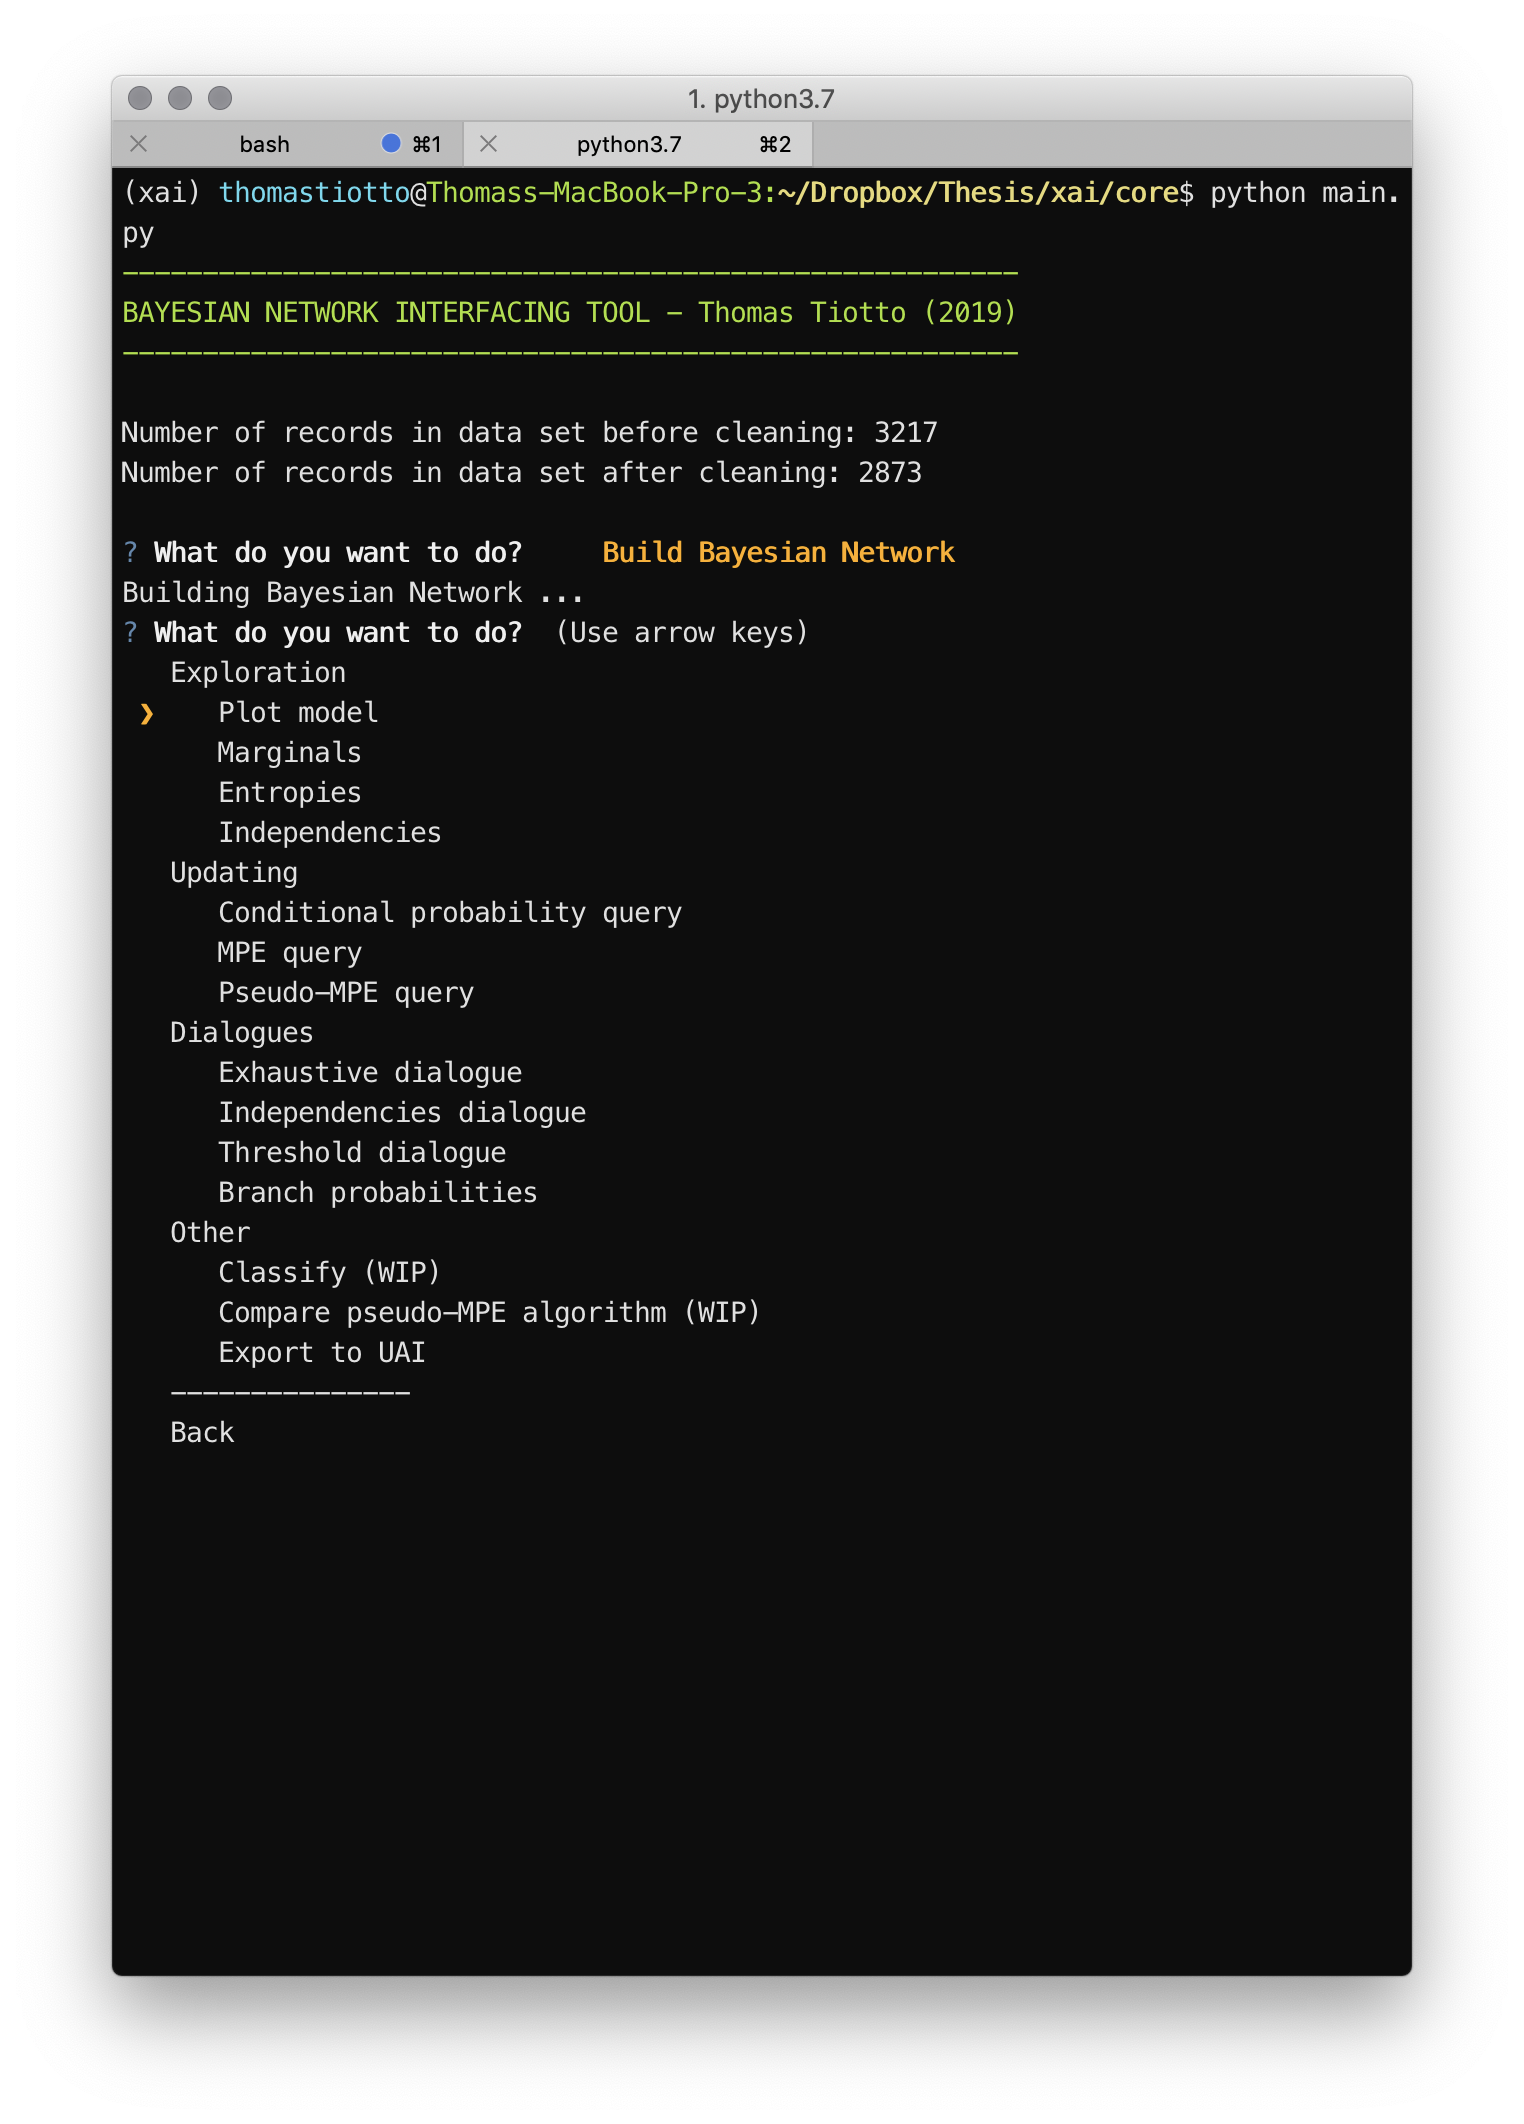
\includegraphics[width=\columnwidth]{results/images/sw_1}}
\caption{Main interaction menu.}
\label{fig:sw_1}
\end{figure}

\subsection{Independencies} \label{subsec:independencies-query}
The \enquote{Independencies} interaction mode gives the expert the possibility of verifying which d-separations (defined in \ref{subsec:d-separation}) exists in the constructed Bayesian Network's DAG (defined in \ref{subsec:graphs}) .
The concept of d-separation is here reworded into a higher-level notion of \enquote{choosing a source variable and a set of evidences to see which other variables have influence on the source, given the evidence}.
This is because Dr. Vittoria Martin, my main contact at the ICP, initially had difficulty in conceptualising at the level of graph theory, probably due the \enquote{false friendliness} with concept of edges and trees. 
Indeed, in clinical practice is quite common deal with this kind of representation; however, the presence of an edge is commonly interpreted not only as a correlation, but also often in a causal mode. 
Thus, the concept of d-separation could be misinterpreted because of the consolidated attitude in front of a tree.
For this same reason, after having chosen first the source variable and then the observed set of evidence variables, the user is presented with an output both in graph (Fig. \ref{fig:independencies_output}) and in natural language (Fig. \ref{fig:sw_2_independencies}) form.
Having both output forms was seen to reduce the confusion associated with such an unfamiliar concept to users trained in the medical sciences.

\begin{figure}[htbp]
\centerline{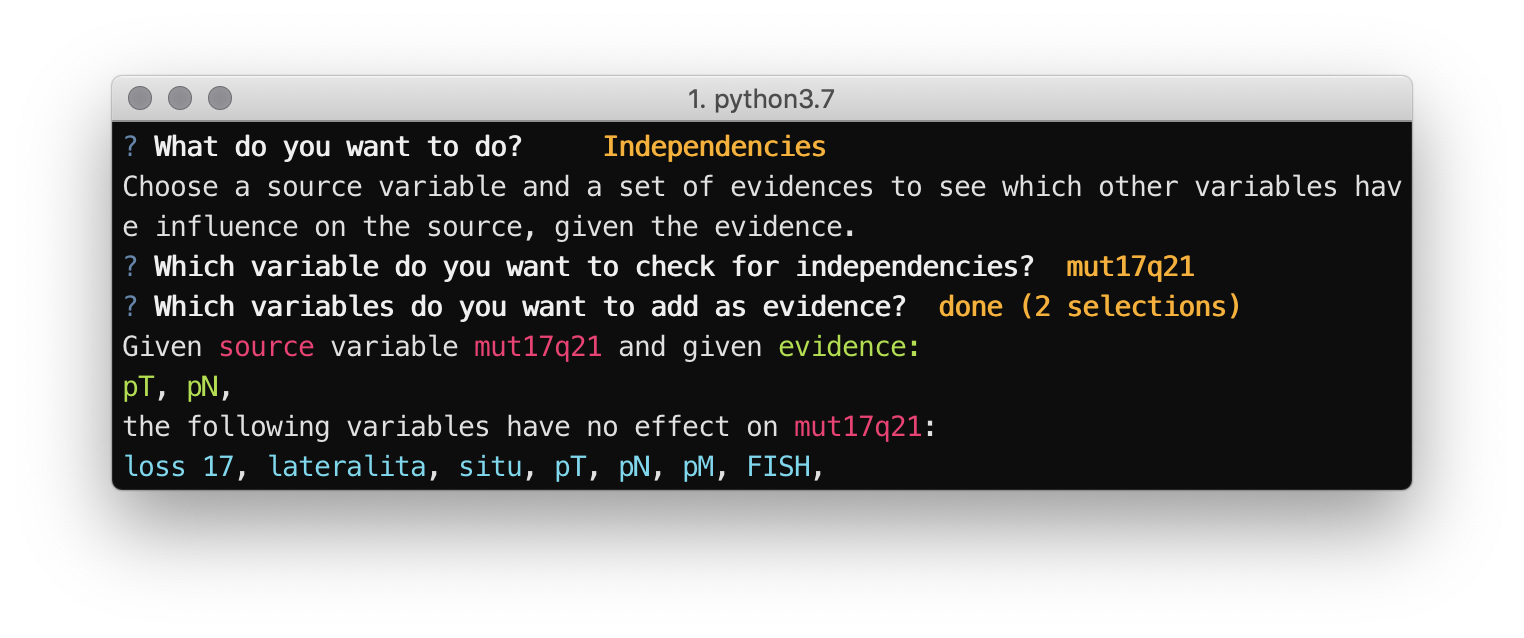
\includegraphics[width=\columnwidth]{results/images/sw_2_independencies}}
\caption{Independencies query natural language output.}
\label{fig:sw_2_independencies}
\end{figure}

\begin{figure}[htbp]
\centerline{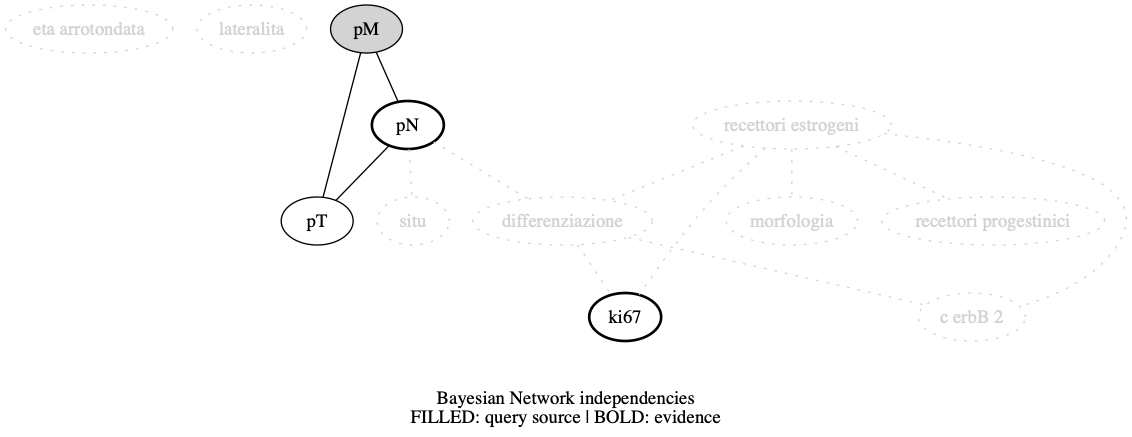
\includegraphics[width=\columnwidth]{results/images/independencies_output}}
\caption{Independencies query graph output.}
\label{fig:independencies_output}
\end{figure}

\subsection{Conditional Probability Query}
Conditional probability queries (defined in Subsec. \ref{subsec:conditional-probabilities}) were seen to be instinctively understood by the clinicians at the ICT.
Indeed, many of the natural language questions that were defined to validate the system (see Sec. \ref{sec:validation}) were naturally instances of this type of query.

The user is asked for a target variable of which to observe the conditioned values and for a set of variables, together with their observed values.
The output, in natural language (Fig. \ref{fig:sw_3_query}), includes all elements of the query in a colour-coded manner.
The answer to the question posed (in cyan) shows the probability of each of the states of the target variable, quantified in natural language, using the coding defined in Tab. \ref{tab:naturallanguageprobabilities}, and as raw probabilities, shown as a percentage.

\begin{figure}[htbp]
\centerline{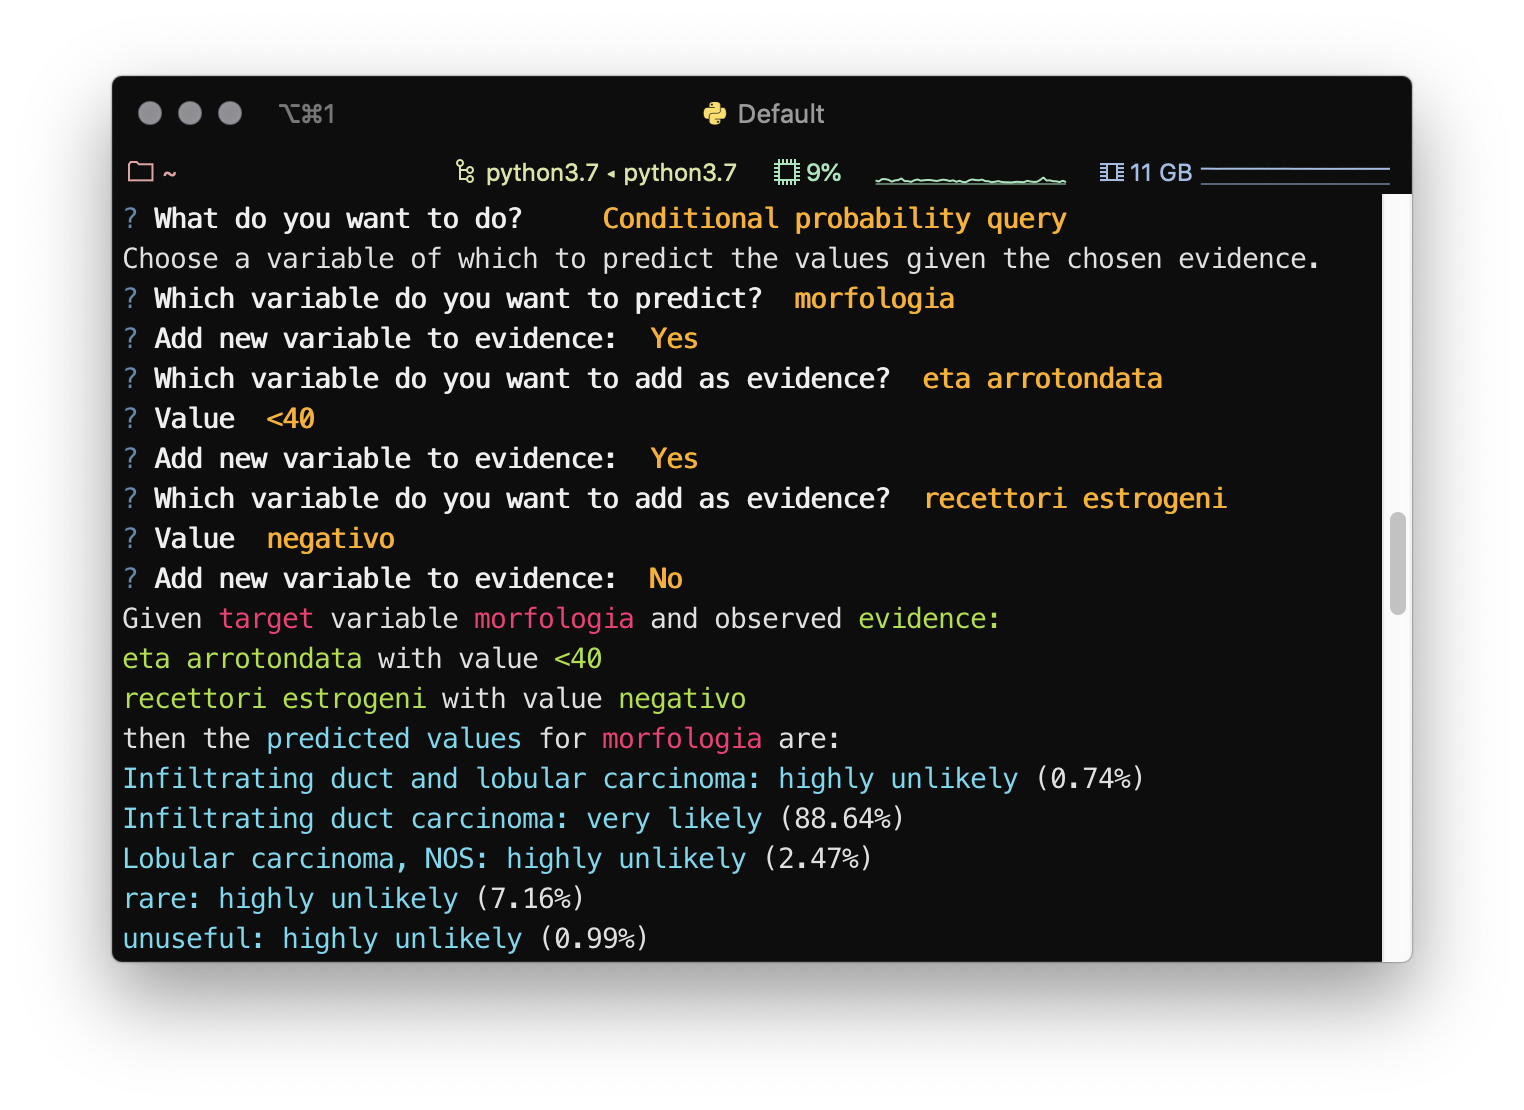
\includegraphics[width=\columnwidth]{results/images/sw_3_query}}
\caption{Conditional probability query output.}
\label{fig:sw_3_query}
\end{figure}

\subsection{MPE Query}
Queries of the MPE type (defined in Subsec. \ref{subsec:bnupdating}) were also understood naturally when a bridge to the clinical practice had been established.
When presented at an abstract, mathematical level, the experts of the ICT weren't clear of the utility of such a query class.
It was soon understood that an MPE query corresponds to a familiar concept to any clinician, that of \enquote{a maximally likely patient profile}.
That is, given a set of known parameters, it is of interest for the expert to find which is the most likely assignment to the other.
As each record in the data set represent a patient's clinical profile, this is equivalent to finding the most probable patient given a set of know values.

Another way than an MPE query makes clinical sense, is in the crucial task of predicting missing values for a patient.
This is not an unlikely case, as discussed in Subsec. \ref{subsec:motivation}, because there is more than one reason that a patient may be missing one or more entries in his clinical profile.
Executing an MPE query with the known patient's values will yield the most probable assignments to the missing ones and is thus equivalent to a prediction task.
The clinical significance of such an interaction mode can also be inferred from the fact that many of the natural language questions that were defined to validate the system (see Sec. \ref{sec:validation}) were seen to map onto instances of this type of query.

At a technical level, the MPE calculation is executed using pgmpy's \texttt{map\_query} function. 
The output, shown in Fig. \ref{fig:sw_4_mpe}, presents in colour-coded natural language the input evidence and most probable assignments to the remaining variables.

\begin{figure}[htbp]
\centerline{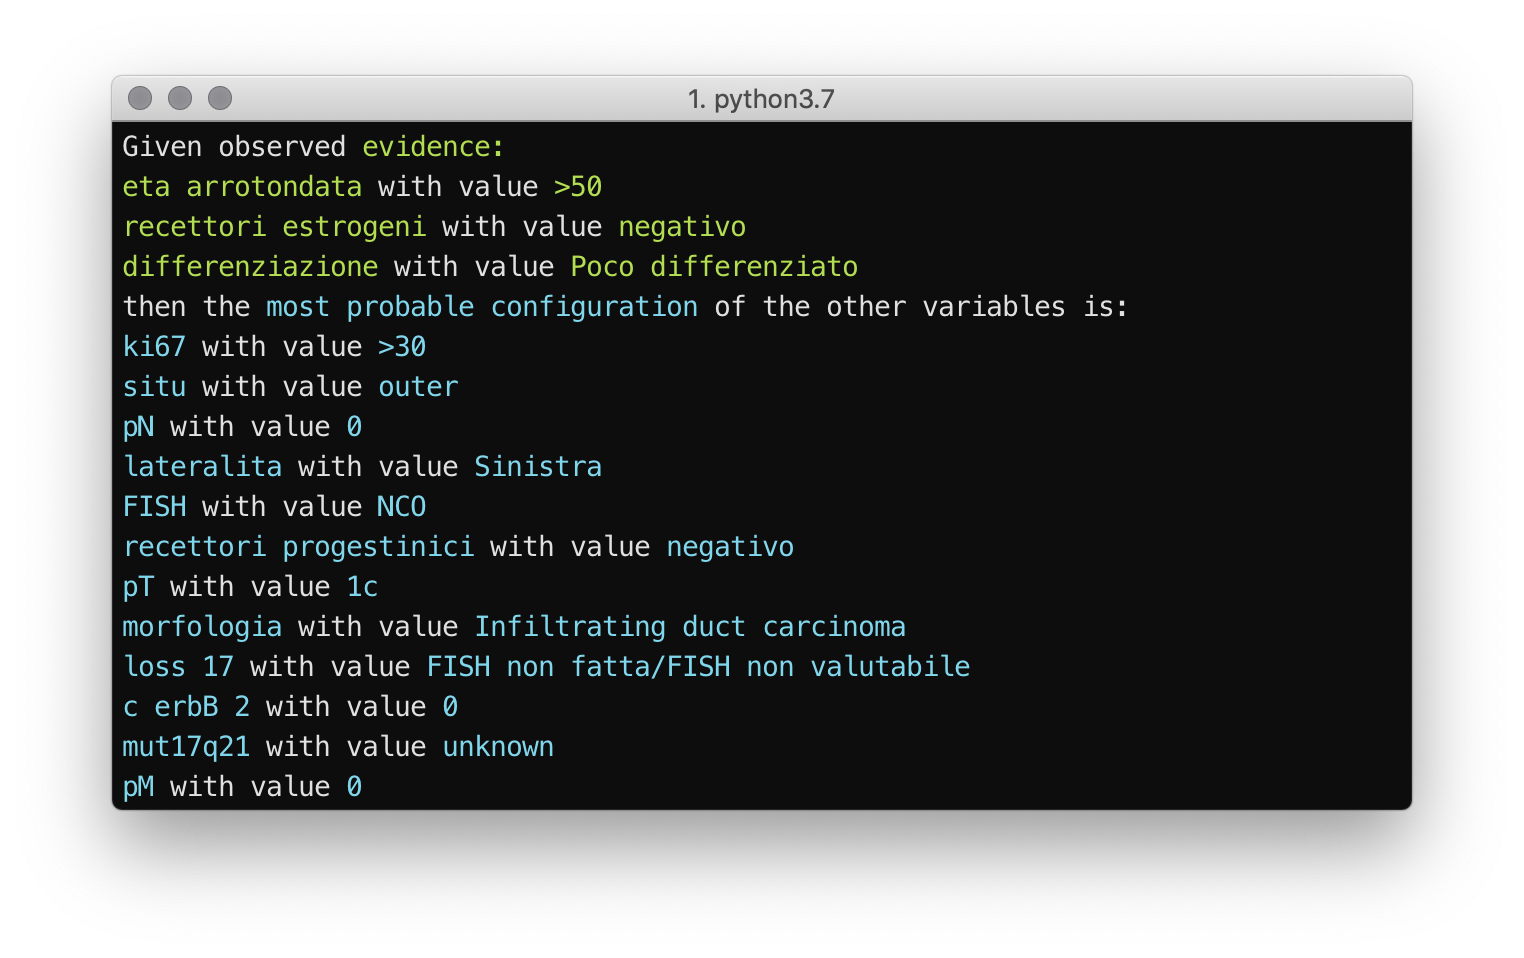
\includegraphics[width=\columnwidth]{results/images/sw_4_mpe}}
\caption{MPE query output.}
\label{fig:sw_4_mpe}
\end{figure}

\subsection{Pseudo-MPE Query}
The \enquote{Pseudo-MPE query} interaction mode is aimed at generating a \textit{max over marginals} assignment using the methods described in Subsec. \ref{subsec:algorithms-novel} under the \textbf{Pseudo-MPE from Initial Evidence} header.
Note that if the cardinality of the set of variables to explain is one, i.e. $|E| = |V|-1$, with $E$ the evidence set and $V$ the set of variables in the BN, then the Pseudo-MPE and true MPE assignments will be identical.

The user is first asked for the probability threshold under which to discard the $(state, value)$ pairs whose probability is deemed too low.
Then, after being asked for the initial observed evidence, the expert is presented with the constructed polytree (defined in Subsec. \ref{subsec:polytrees}), an example of which can be seen in Fig. \ref{fig:pseudo_mpe_output}.
This polytree will have the initial evidences, that the expert specified, as roots and a single chain of $(state, value)$ pairs, each one being quantified with its probability (in natural language) given all of its ancestors.

\begin{figure}[htbp]
\centerline{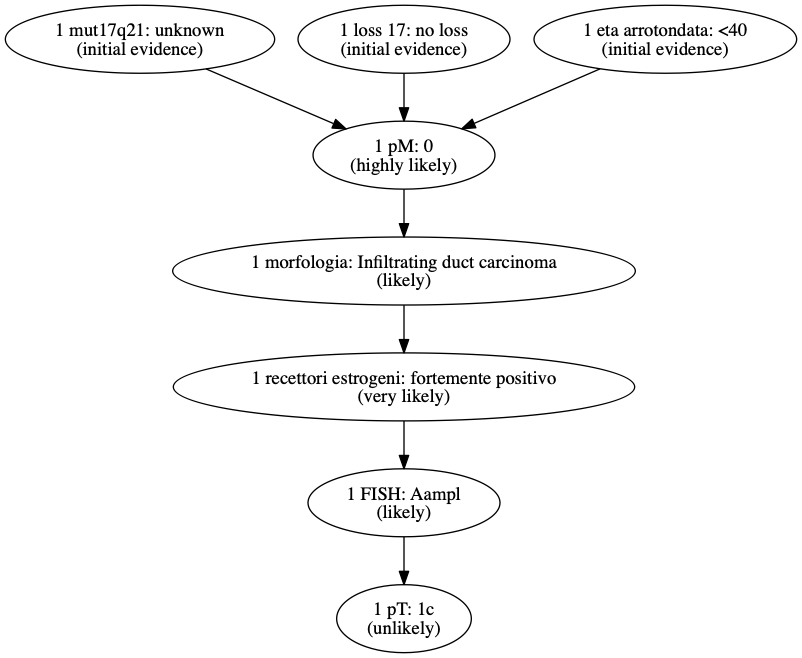
\includegraphics[width=\columnwidth]{results/images/pseudo_mpe_output}}
\caption{Pseudo-MPE query output with threshold $0.5$.}
\label{fig:pseudo_mpe_output}
\end{figure}

\subsection{Exhaustive Dialogue}
The three \enquote{dialogue} are the most experimental interaction modes and thus also the most alien to an expert user.
None of the natural language questions defined by the ICT in form form described in \ref{subsec:clinical-validation-methodology} could be directly mapped onto such a dialogical process.
Because of the novel nature of such a knowledge-extraction process, three different versions were implemented, with each one adding a different set of behaviours, compared to the Exhaustive version described in this subsection.
This let me better explore the space of possibilities and understand which features were preferred by the clinicians of the ICT, both as a means for knowledge-extraction from the data set and from a comprehensibility point of view.
It should here be noted that comprehensibility of the outputs is a \textit{necessary} but not sufficient condition to be able to gain knowledge from data.
Both the variants, the independencies-aware one and the thresholded one, aim to prune the space of variables proposed to the user, in order to reduce her cognitive load.

The Exhaustive Dialogue, as described in much more detail in Subsec. \ref{subsec:algorithms-novel} under the \textbf{Dialogues} header, is so named because it ends only when the expert user has reviewed all the variables present in the data set.
It starts by asking the clinician for a set of initial evidences and from thereon-after iteratively proposes the least entropic $(state,value)$ pair, based on the accumulated evidence (the rationale behind this is explained in Subsec. \ref{subsec:entropy-based-selection}).
An example of such an ongoing interaction is shown in Fig. \ref{fig:sw_5_exhaustive_dialogue}.

\begin{figure}[htbp]
\centerline{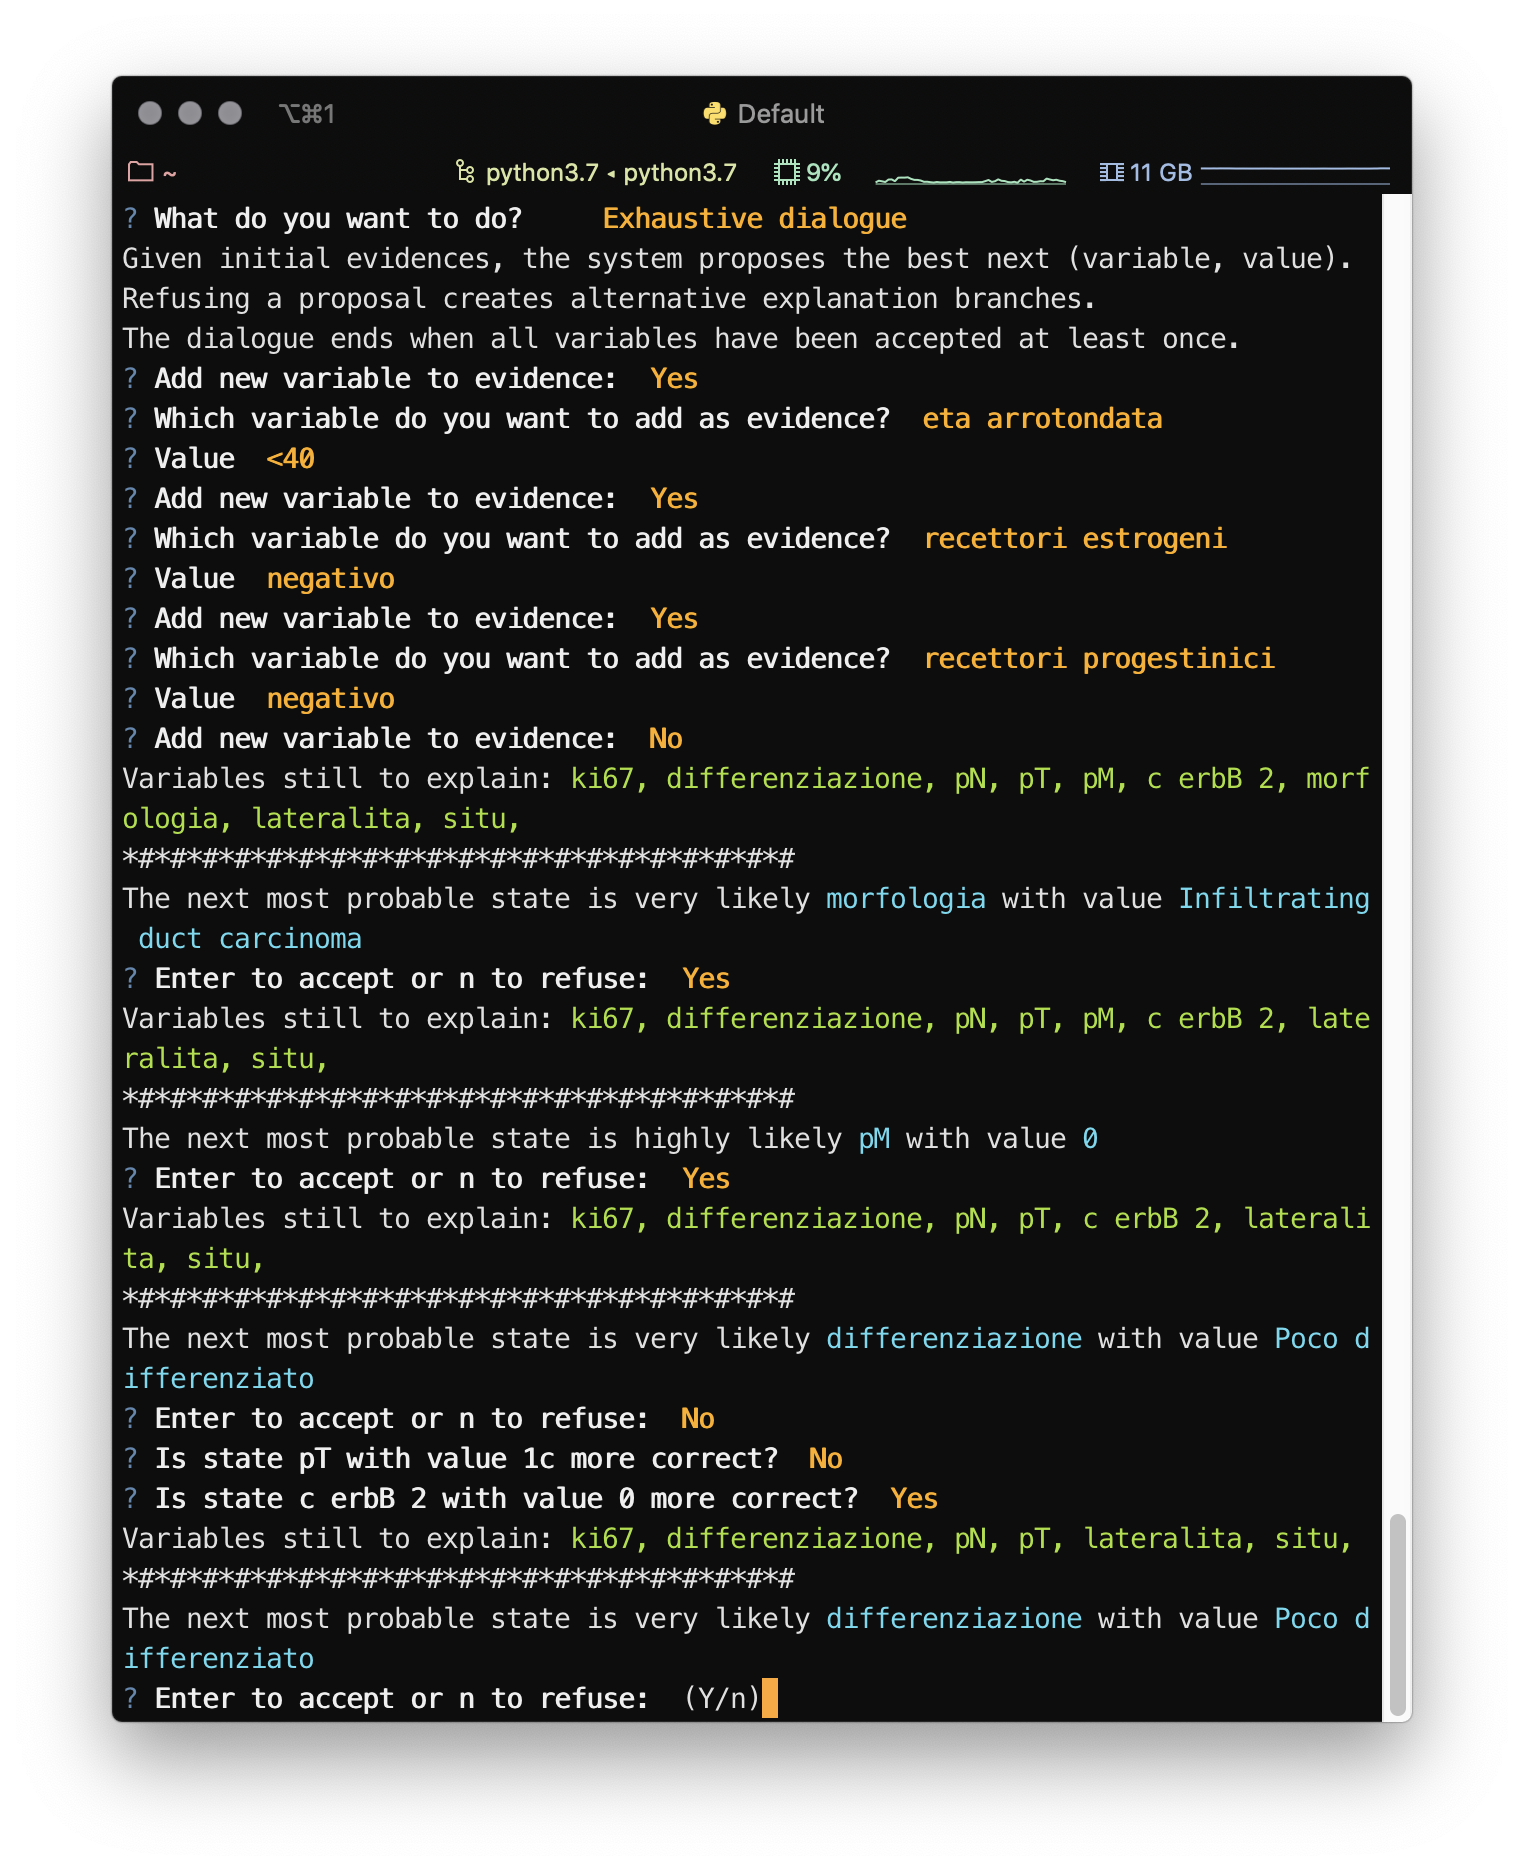
\includegraphics[width=\columnwidth]{results/images/sw_5_exhaustive_dialogue}}
\caption{Ongoing Exhaustive Dialogue.}
\label{fig:sw_5_exhaustive_dialogue}
\end{figure}

\subsection{Independencies Dialogue}
The first variant to the Exhaustive Dialogue takes the approach of excluding variables based on their d-separations (defined in Subsec. \ref{subsec:d-separation}) in the underlying DAG (defined in Subsec. \ref{subsec:graphs}).
Thus, in the general case, the cardinality of set of variables proposed to the user varies in a non-linear way.
In the Exhaustive Dialogue, presented under the previous header, the relationship between the set of variables still to explain at step $t$ $W_t = V \setminus E_t$, with $V$ all the variables and $E_t$ those already added to evidence, obeyed the recurrence relation:
\begin{align}
	W_0 := V \\
	E_0 := \emptyset \\
	|W_{t+1}| = |W_t| - 1 \\
	|E_{t+1}| = |E_t| + 1
\end{align}
That is, at each step $t$ of the Exhaustive Dialogue, one variable moves from the set still to explain $W$ to the explained one $E$.
In the Independecies Dialogue, this relationship depends on the set of variables $Z$ that are d-separated from those already in $E$.
The relationship between the cardinalities is modelled by an operator $\zeta$ that is unique to the DAG of the BN (or to any \textit{I-equivalent} one):
\begin{align}
	W_0 := V \\
	E_0 := \emptyset \\
	|W_{t+1}| = \zeta(|E_t|) \\
	|E_{t+1}| = |E_t| + 1
\end{align}
As d-separation is not monotonic (adding a variable to $E$ may open new paths), the cardinality of the set $W$ may vary, from the point of view of the user, in an unpredictable manner.
The user is supported by an updated view of the independencies in the graph (an example during the dialogue is shown in Fig. \ref{fig:independencies_dialogue_output}.

Before receiving feedback from the ICT, the visualisation of the independencies was the one shown in Fig. \ref{fig:independencies_dialogue_output_old}.
The most striking difference was the use of colour-coding to identify the role and the separateness of variables with pink identifying the query variables, blue the evidences, red the separated variables and green the connected ones.
As already noted in Subsec. \ref{subsec:independencies-query}, the concept of d-separation turned out to be quite unfamiliar to the clinicians of the ICT so the first priority was to represent the concept visually in the clearest way possible.
This was achieved, and confirmed in its efficacy by the ICT, by fading the separated variables and marking those in evidence in bold, as can be seen in Fig. \ref{fig:independencies_dialogue_output}.

A second point of confusion, that hadn't been foreseen, was the use of directed arcs to represent the DAG.
In the visual representation of a Bayesian Network, an arc between two variables represents a correlation between their values while the direction identifies the $parent$ and the $child$ in the relationship; for example the graphical representation $X \rightarrow Y$ means that $X$ is the parent of $Y$.
This is crucial because the fundamental idea of a BN model is to factorise the joint distribution such that each variable's values depend only on that of its parents; the concept of Conditional Probability Table is explained in Sec. \ref{sec:bayesiannetworks} and a some more examples can be seen in Subsec. \ref{subsec:algorithms} under the \textbf{MPE} header.
Nonetheless, Dr. Vittoria Martin explained that the DAG representing a BN is very similar to diagrams used during clinical research, with the crucial difference that in those a directed arrow represents \textit{causation} and not \textit{correlation}.
A correlative relationship would have usually been represented by an undirected edge.
For this reason, I elected to substitute the DAG representation of the BN with that of an undirected graph.
The ICT representative confirmed that this aligned much better with her intuition.

The third element of difference, is the addition of the Mutual Information coefficient (defined in Subsec. \ref{subsec:mutualinformation}) on the arcs connecting each couple of variables; the coefficient also scales the width of its associated edge, giving further visual feedback to the user.
This was a direct request from the ICT's representatives as they felt that this would increase their understanding of the relationships between the variables.
D-separation is binary while Mutual Information can give the practitioner a much greater (theoretically, infinite) range of information.
For example looking at Fig. \ref{fig:independencies_dialogue_output} it is quite easy to see that, while \enquote{morfologia} and \enquote{recettori estrogeni} are d-connected, the amount to which they influence each other's values is small, compared to other connected variables.
Some arcs, for example those belonging to \enquote{mut17q21}, are missing the Mutual Information coefficient because either the parent or the child variable is in the evidence set.

\begin{figure}[htbp]
\centerline{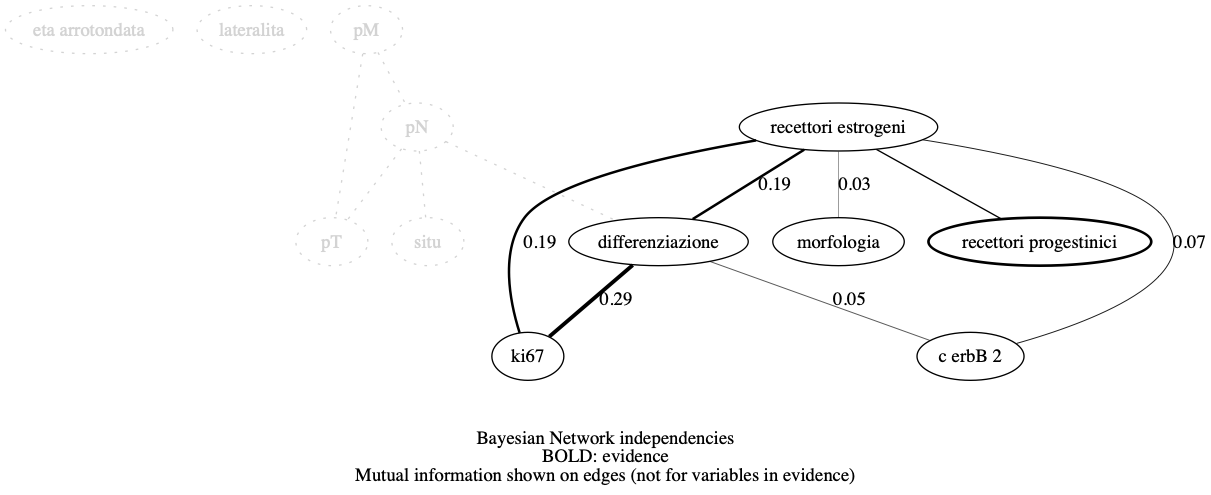
\includegraphics[width=\columnwidth]{results/images/independencies_dialogue_output}}
\caption{Ongoing Independencies Dialogue.}
\label{fig:independencies_dialogue_output}
\end{figure}

\begin{figure}[htbp]
\centerline{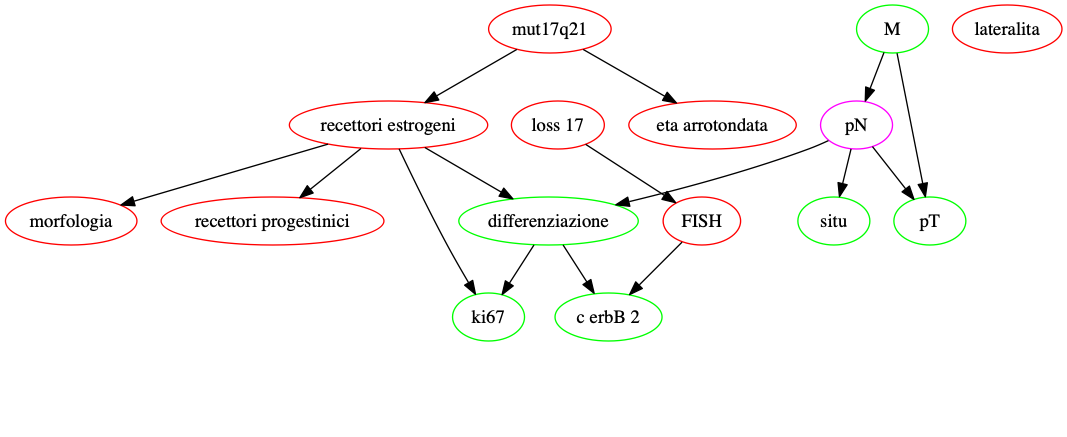
\includegraphics[width=\columnwidth]{results/images/independencies_dialogue_output_old}}
\caption{Old visualisation during Independencies Dialogue.}
\label{fig:independencies_dialogue_output_old}
\end{figure}

\subsection{Threshold Dialogue}
The final Dialogue variant adopts a different strategy for pruning, namely one based on the probability of the proposed tuples and on the number of times that they have been refused by the expert.
The cardinality of the set $W$ of states to explain decreases linearly, like in the Exhaustive Dialogue, but potentially with a slope coefficient $\alpha \leq -1$, as many states may be infra-threshold i.e. too unprobable to be considered.
Unlike the Independencies Dialogue, the cardinality of $W$ can't increment:
\begin{align}
	W_0 := V \\
	E_0 := \emptyset \\
	|W_{t+1}| = \alpha |W_t| \\
	|E_{t+1}| = |E_t| + 1
\end{align}
The default values for the threshold and the maximum number of times a $(state, value)$ tuple could be proposed, were decided together with the ICT and set to xx and xx, respectively.

\subsection{Combination of Features from All Dialogue Variants}

